% Introdução

\documentclass[_ArquivoPrincipal.tex]{subfiles}

\begin{document}

%==================================================================================================
\chapter{Estado Da Arte}
%==================================================================================================
	
No presente capítulo serão abordados os principais temas relacionados à problemas de Interação Fluido-Estrutura (IFE), tendo como ênfase os modos de turbulência. Serão destacados os principais métodos de cálculos envolvendo a dinâmica das estruturas computacional (\ref{CSD}), a dinâmica dos fluidos computacional (\ref{CFD}), modo de acoplamento Lagrangiana-Euleriana Arbitrária (\textit{Arbitrary Lagrangian-Eulerian} - ALE) (\ref{ALE}) e alguns modelos de turbulências (\ref{MT}).

%==================================================================================================
\section{Dinâmica Das Estruturas Computacional} \label{CSD}
%==================================================================================================

A mecânica dos sólidos visa a determinação de parâmetros referentes à elementos estruturais sujeitos a solicitações externas, tais como tensões e deformações, ou forças e deslocamentos de determinados pontos dos mesmos. Para isso são desenvolvidos diversos métodos com a finalidade de melhor descrever o comportamento das estruturas, como o Método dos Elementos Finitos (MEF), que se apresenta como a ferramenta computacional mais amplamente utilizada para esse fim.

Nesse sentido vale ressaltar os trabalhos de \citeonline{hughes1981nonlinear, argyris1982excursion, ibrahimbegovic2002role, pimenta2004fully, battini2006choice} e \citeonline{pimenta2008exact}, que realizaram análises através do MEF Corrotacional, que se trata de uma formulação onde os deslocamentos e rotações dos elementos são os parâmetros principais da análise.

No entanto a utilização de uma análise que considera tais parâmetros nodais só se mostra eficiente ao se estudar estruturas que desenvolvem pequenos deslocamentos e deformações. Isso deve-se ao fato de essa abordagem utilizar rotações finitas como parâmetros nodais, o que pode gerar controversas em problemas envolvendo grandes rotações, uma vez que não há comutatividade entre essas grandezas \cite{sanches2013unconstrained}. Ainda observa-se que a avaliação dinâmica de estruturas reticuladas se torna problemática, do ponto de vista da conservação de energia \textcolor{red}{(COMENTAR MAIS) (REFERÊNCIAS)}, além da matriz de massa ser variável, tornando o processo de integração temporal muito complexo.

Com isso, vale ressaltar os trabalhos de \citeonline{coda2004simple, coda2007alternative, coda2010improved, coda2009two, coda2009unconstrained} e \citeonline{carrazedo2010alternative} que utilizam de forma bem-sucedida o MEF Posicional para análise de estruturas reticuladas e de cascas aplicadas à grandes deslocamentos. Este método se diferencia dos demais ao considerar as posições nodais, obtidas a partir de vetores indeformados, como parâmetros de análise, facilitando o cálculo de efeitos de não-linearidade geométrica.

\citeonline{sanches2013unconstrained} apresentaram uma aplicação do método dos elementos finitos posicional em elementos de cascas e constataram a presença de uma matriz de massa constante, o que possibilita a utilização de métodos de integração temporal, como o método de Newmark $\beta$, conservando, assim, o momento linear e angular em análises dinâmicas. Além disso, esse trabalho também analisou problemas envolvendo IFE, obtendo resultados favoráveis, indicando a boa aplicação desse método em problemas dessa natureza.

No âmbito da IFE, destaca-se a necessidade dessa consideração, uma vez que são observadas aplicações como, por exemplo, grandes amplitudes de deslocamentos, como \textit{flutter} \textcolor{red}{(REFERÊNCIAS)}, aplicações biomecânicas \textcolor{red}{(REFERÊNCIAS)}, estruturas infláveis \cite{karagiozis2011computational}, simulações de turbinas \cite{bazilevs20113d}, dentre outras.

%==================================================================================================
\section{Dinâmica Dos Fluidos Computacional} \label{CFD}
%==================================================================================================

Ao contrário de problemas envolvendo elementos sólidos, que possuem um estado inicial bem definido, os fluidos, em especial os Newtonianos, não o possuem, uma vez que não incapazes de resistir à tensões desviadoras, deformando-se, assim, indefinidamente quando sujeitos à essas tensões. Dessa forma, torna-se apropriada a utilização de uma descrição Euleriana para descrever os fluidos, em que os parâmetros nodais são principalmente as velocidades do mesmo \textcolor{red}{(REFERÊNCIAS)}.

Em geral, problemas envolvendo Dinâmica dos Sólidos (\textit{Computational Solid Dynamics} - CSD) partem do princípio da estacionariedade de energias, buscando a determinação do ponto em que a energia do sistema seja mínima. Isso proporciona uma diversidade de métodos, como o Princípio dos Trabalhos Virtuais (PTV) o método de Galerkin, o método de Ritz, dentre outros. Esses métodos apresentam a particularidade de surgir um sistema de equações com uma matriz simétrica e, em alguns casos, de vetores cujas componentes possuem significado físico. Porém, em problemas que envolvem a Dinâmica dos Fluidos (\textit{Computational Fluid Dynamics} - CFD), o sistema de equações possui uma matriz, na maioria dos casos, assimétrica, devido à presença de termos convectivos nas equações governantes.

Nesse sentido, são desenvolvidos novos métodos, em busca de uma solução mais representativa com uma malha menos refinada. Dentre os pricipais desenvolvidos, vale mencionar o \textit{Streamline-Upwind/Petrov-Galerkin} (SUPG) \textcolor{red}{(REFERÊNCIAS)}, \textit{Galerkin Least-Squares} (GLS) \textcolor{red}{(REFERÊNCIAS)}, \textit{Subgrid Scales} (SGS) \textcolor{red}{(REFERÊNCIAS)} e \textit{Consistent Approximate Upwind} (CAU) \textcolor{red}{(REFERÊNCIAS)} \textcolor{red}{COMENTAR SOBRE OS MÉTODOS}.

Um campo que vale destacar na CFD é o que estuda os fenômenos de turbulência, uma vez que esses fenômenos podem se apresentar nas mais variadas escalas, sendo necessário a geração de uma malha muito refinada para detectar a formação dos vórtices, o que ocasiona um aumento radical no custo computacional da análise. Assim, são desenvolvidas novas técnicas afim de se obter melhores resultados, sem que haja um grande aumento no volume de cálculos. Dentre esses métodos destacam-se os métodos multiescala (\textit{Variational Multiscale Methods} - VMS), as simulações de grandes vórtices (\textit{Large Eddy Simulation} - LES) \textcolor{red}{(REFERÊNCIAS)}, os métodos de atualização de malha (\textit{Remeshing}) \textcolor{red}{(REFERÊNCIAS)} e aproximações de \textit{Reynolds-Averaged Navier-Stokes} \textcolor{red}{(REFERÊNCIAS)}. O item \ref{MT} descreve de forma mais detalhada cada um desses métodos.

%==================================================================================================
\section{Modelo De Turbulência} \label{MT}
%==================================================================================================

Um fluido pode apresentar um escoamento de duas formas distintas, a depender do número de Reynolds que este apresenta (conforme ilustrado na Figura \ref{fig:Escoamentos}). Em casos cujo número de Reynolds é baixo, o escoamento é considerado laminar, ou seja, o escoamento se dá de forma semelhante ao movimento de lâminas independentes, não havendo mistura mascroscópica entre as mesmas. Já em casos cujo número de Reynolds é muito elevado, o escoamento é considerado turbulento. Nesse cenário há a formação de vórtices sobre o escoamento, que podem ocorrer de forma instável e em várias escalas diferentes. Esse fenômeno pode ser descrito de acordo com as equações de Navier-Stokes, no entanto sua resolução se apresenta com um alto grau de complexidade, uma vez que possui termos não lineares em sua composição. Assim são necessárias técnicas de solução, para que se possa obter uma solução de forma aproximada à essas equações. Os itens que seguem apresentam algumas técnicas utilizadas para esse fim.

\begin{figure}[h]
    \centering
    \begin{subfigure}{.45\textwidth}
        \centering
        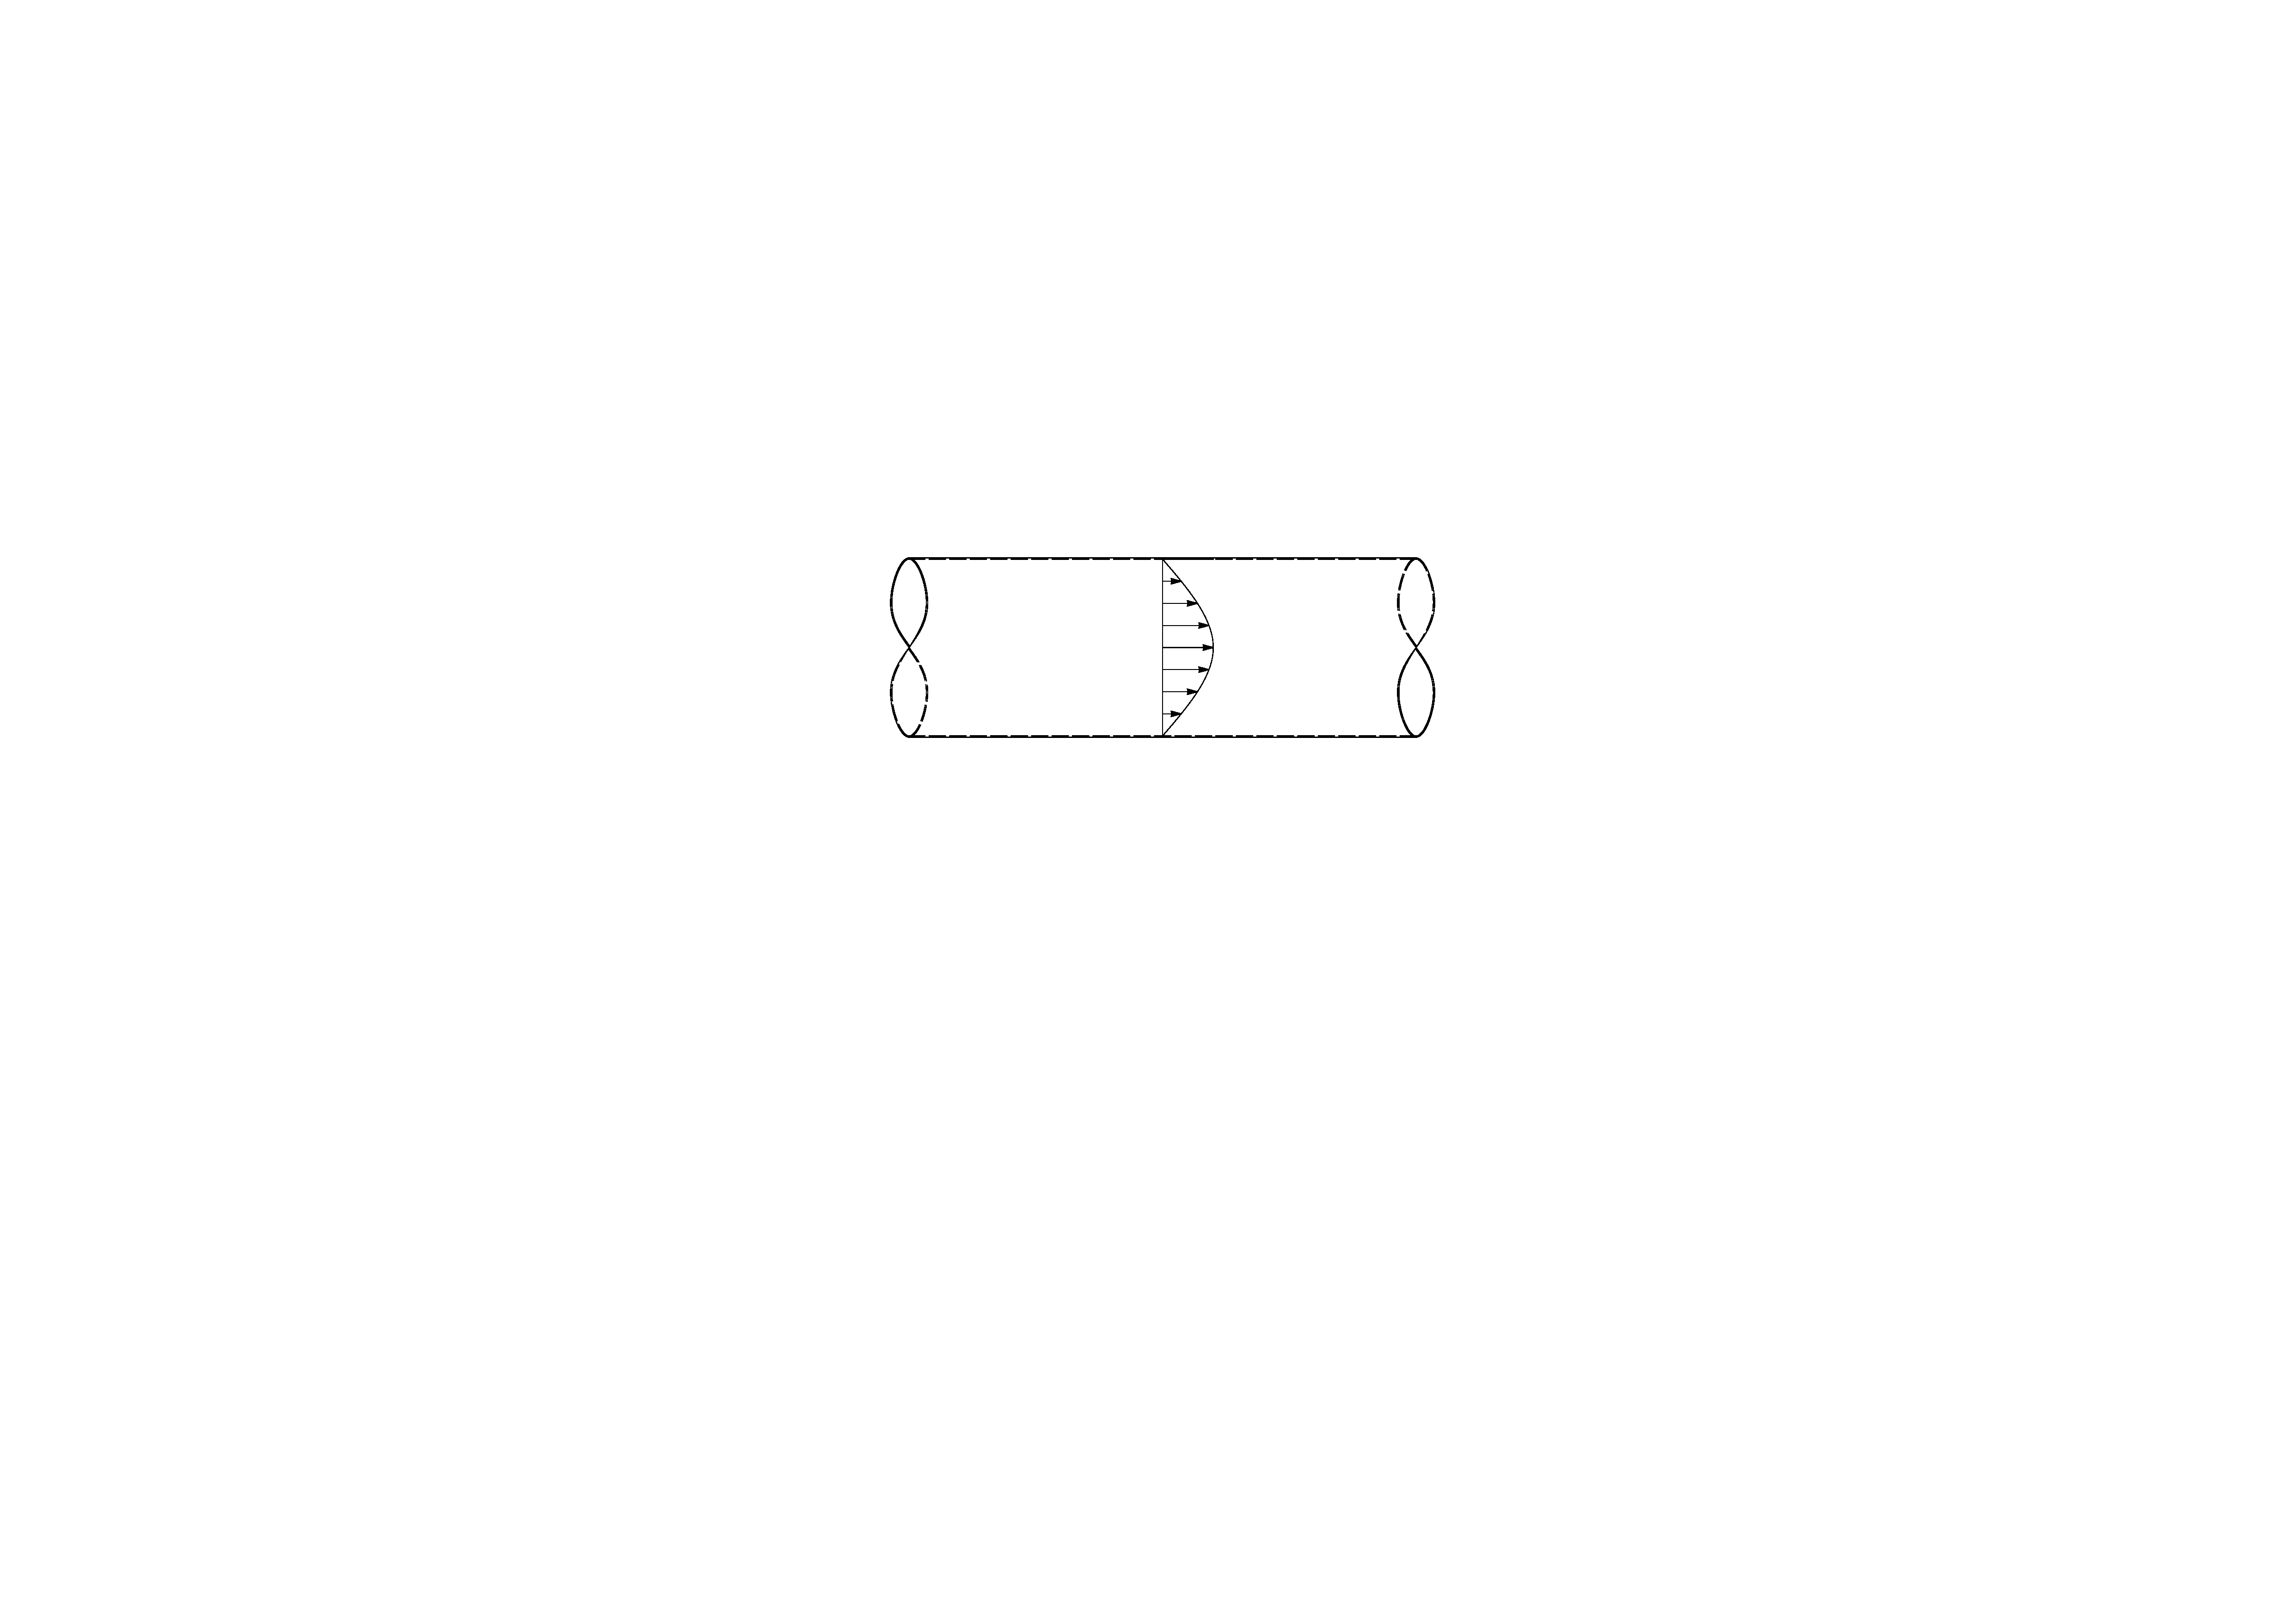
\includegraphics[width=\linewidth]{Figuras/EscLaminar.pdf}
        \caption{Escoamento laminar.}
        \label{fig:EscLaminar}
      \end{subfigure}
      \begin{subfigure}{.45\textwidth}
        \centering
        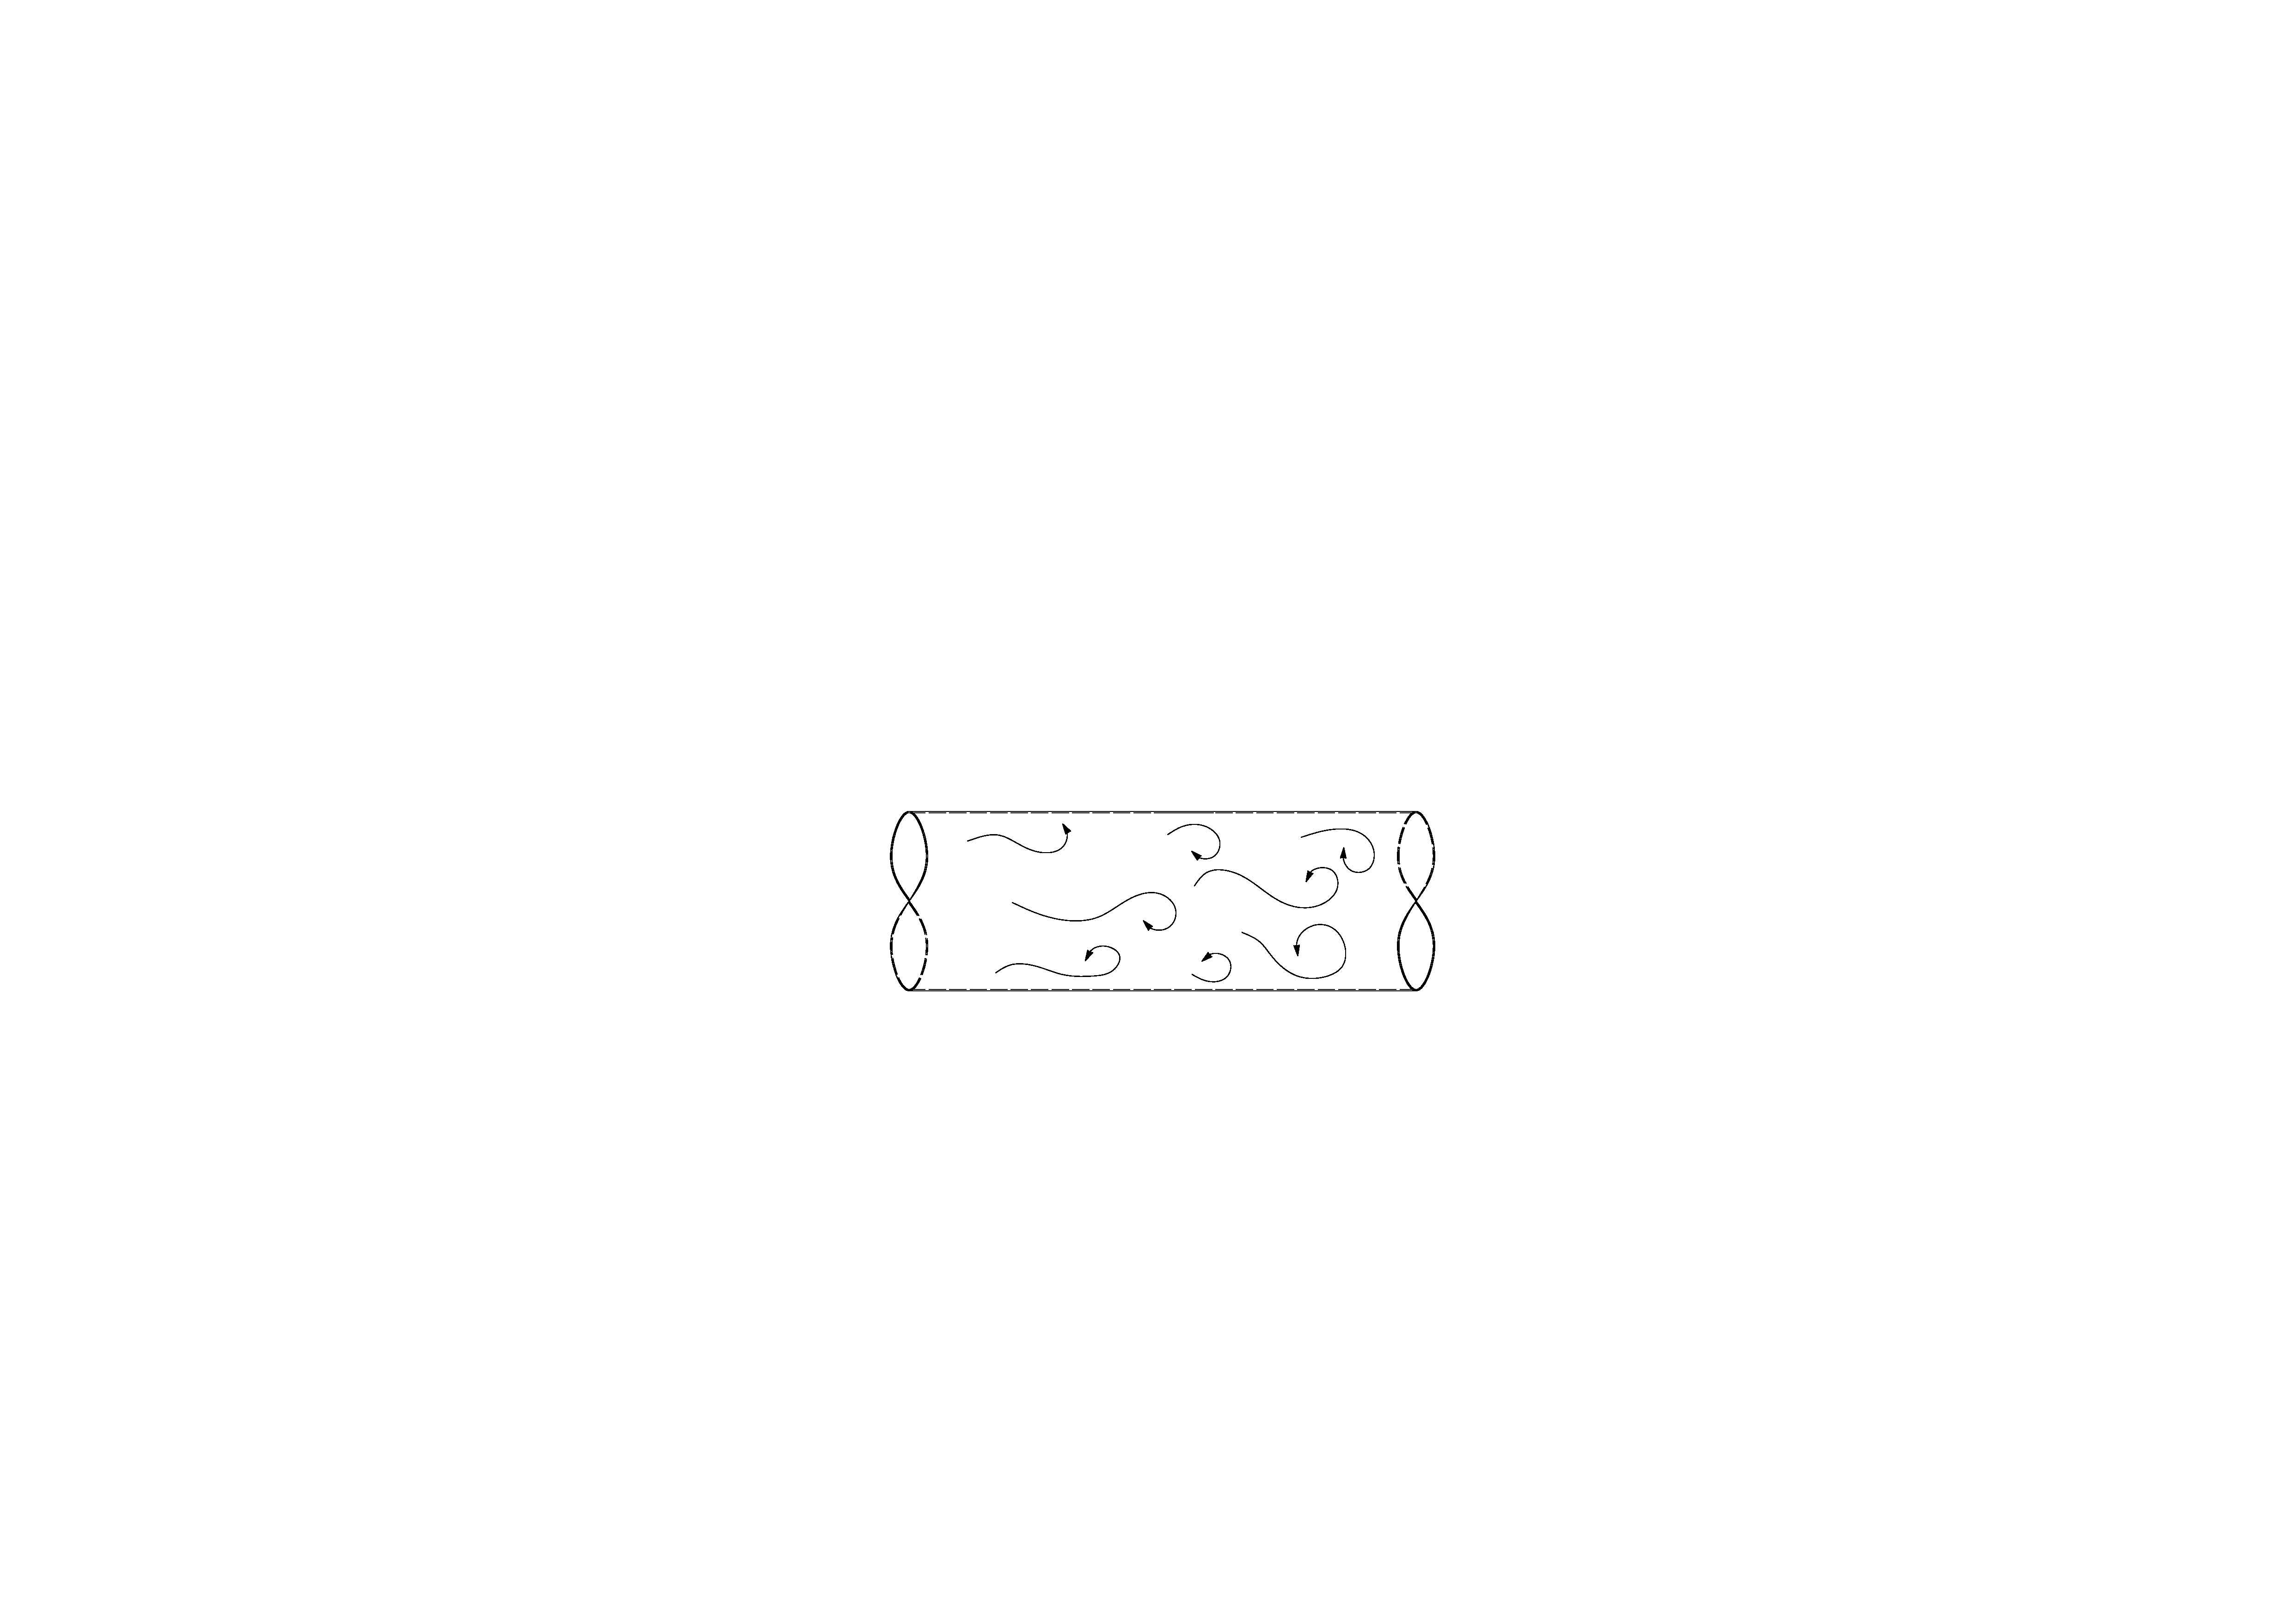
\includegraphics[width=\linewidth]{Figuras/EscTurbulento.pdf}
        \caption{Escoamento turbulento.}
        \label{fig:EscTurbulento}
      \end{subfigure}
    \caption{Esquema de escoamentos.\label{fig:Escoamentos}}
\end{figure}

%==================================================================================================
\subsection{Equações Governantes da Dinâmica dos Fluidos} \label{EqGov}
%==================================================================================================

As equações de Navier-Stokes são equações diferenciais parciais, cuja resolução resulta na obtenção de campos de velocidades ($\mathbf{u}$) e de pressões ($p$). Para obtenção dessas equações é considerado um fluido newtoniano em escoamento incompressível, em regime turbulento (alto número de Reynolds) e a temperatura constante. Levando-se em consideração os princípios da conservação da massa, que em descrição Euleriana pode ser escrita de acordo com a Equação \ref{ConMas1}, ou Equação \ref{ConMas2}:

\begin{equation}
    \left.\frac{\partial\rho}{\partial t}\right|_{\mathbf{y}}+\mathbf{\nabla}_\mathbf{y}\cdot(\rho\mathbf{u})=0\text{, ou}
    \label{ConMas1}
\end{equation}
\begin{equation}
    \frac{D\rho}{Dt}+\rho\mathbf{\nabla}_\mathbf{y}\cdot\mathbf{u}=0\text{,}
    \label{ConMas2}
\end{equation}

\noindent em que $\rho$ representa a massa específica do fluido e $D\rho/Dt$ representa a derivada material, dada por:

\begin{equation}
    \frac{D\rho}{Dt}=\left.\frac{\partial\rho}{\partial t}\right|_\mathbf{y}+\mathbf{u}\cdot\mathbf{\nabla}_\mathbf{y}\rho\text{,}
    \label{DerMat}
\end{equation}

\noindent pode-se obter que 

\begin{equation}
    \mathbf{\nabla}_\mathbf{y}\cdot\mathbf{u}=0\text{,}
    \label{Divu0}
\end{equation}

\noindent para fluidos em escoamento incompressível.

Já a conservação da quantidade de movimento pode ser escrita como:

\begin{equation}
    \left.\frac{\partial(\rho\mathbf{u})}{\partial t}\right|_\mathbf{y}+\mathbf{\nabla}_\mathbf{y}\cdot(\rho\mathbf{u}\otimes\mathbf{u})-\mathbf{\nabla}_\mathbf{y}\cdot\mathbf{\sigma}-\mathbf{b}=\mathbf{0}\text{,}
    \label{ConQuantMov}
\end{equation}

\noindent em que $\mathbf{b}$ representa as forças de volume atuantes no fluido e $\mathbf{\sigma}$ representa o tensor de tensões viscosas, que segue o modelo constitutivo para fluidos como \ref{ConstLaw1}:

\begin{equation}
    \mathbf{\sigma}=\mathbf{\tau}-p\mathbf{I}\text{,}
    \label{ConstLaw1}
\end{equation}

\noindent na qual $\mathbf{I}$ é o tensor identidade e $\mathbf{\tau}$ é o tensor de tensões desviadoras, que pode ser obtido como:

\begin{equation}
    \mathbf{\tau}=\lambda\mathbf{I}\textrm{tr}(\dot{\mathbf{\varepsilon}})+2\mu\dot{\mathbf{\varepsilon}}\text{,}
    \label{TensDesv}
\end{equation}

\noindent sendo $\mu$ a viscosidade cinemática do fluido e $\dot{\mathbf{\varepsilon}}$ a taxa de deformação infinitesimal, dada por:

\begin{equation}
    \dot{\mathbf{\varepsilon}}=\frac{1}{2}\left(\mathbf{\nabla}^T_\mathbf{y}\mathbf{u}+\mathbf{\nabla}_\mathbf{y}\mathbf{u}\right)\text{.}
    \label{TaxaDef}
\end{equation}

Dessa forma, substituindo-se as equações \ref{Divu0}, \ref{ConstLaw1}, \ref{TensDesv} e \ref{TaxaDef} em \ref{ConQuantMov} e fazendo as devidas simplificações, obtém-se a Equação \ref{NavierStokes}:

\begin{equation}
    \frac{\partial\mathbf{u}}{\partial t}+\mathbf{\nabla}_\mathbf{y}\cdot(\mathbf{u}\otimes\mathbf{u})+\mathbf{\nabla}_\mathbf{y}\tilde{p}=\nu\mathbf{\nabla}^2_\mathbf{y}\mathbf{u}+\tilde{\mathbf{b}}\text{,}
    \label{NavierStokes}
\end{equation}

\noindent na qual $\nu$ é a viscosidade dinâmica do fluido, $\tilde{p}$ é a pressão dividida pela massa específica do fluido e $\tilde{\mathbf{b}}$ é a força de volume dividida pela massa específica do fluido.

Para $\mu>0$, as equações \ref{Divu0} e \ref{NavierStokes} são denominadas como Equações de Navier-Stokes para escoamento incompressível, enquanto para $\mu=0$ as equações são denominadas de Equações de Euler.

Nesse sentido, considere um subconjunto aberto $\Omega\in\mathbb{R}^d$, o qual refere-se ao domínio espacial do problema analisado, em que $d$ é o número de dimensões do espaço. Assim, $\Omega$ possui uma fronteira suave $\Gamma=\partial\Omega$ e é analisado em um intervalo de tempo $(0,T)$, no qual $T>0$ representa o tempo final da análise.

Com isso pode-se definir o domínio de tempo-espaço como $\mathrm{Q}=\Omega\times(0,T)$ e $\mathrm{P}=\Gamma\times(0,T)$ como a fronteira do domínio. Assim, o problema pode ser descrito em termos da velocidade $\mathbf{u}:\bar{\mathrm{Q}}\to\mathbb{R}^d$ e da pressão $\bar{p}:\mathrm{Q}\to\mathbb{R}$ como \cite{hughes2000large}:

\begin{equation}
    \frac{\partial\mathbf{u}}{\partial t}+\mathbf{\nabla}_\mathbf{y}\cdot(\mathbf{u}\otimes\mathbf{u})+\mathbf{\nabla}_\mathbf{y}\tilde{p}=\nu\mathbf{\nabla}^2_\mathbf{y}\mathbf{u}+\tilde{\mathbf{b}}\text{, em }\mathrm{Q}\text{,}
    \label{Sist1}
\end{equation}

\begin{equation}
    \mathbf{\nabla}_\mathbf{y}\cdot\mathbf{u}=0\text{, em }\mathrm{Q}\text{,}
    \label{Sist2}
\end{equation}

\begin{equation}
    \mathbf{u}=0\text{, em }\mathrm{P}\text{, e}
    \label{Sist3}
\end{equation}

\begin{equation}
    \mathbf{u}(0^+)=\mathbf{u}(0^-)\text{, em }\mathrm{\Omega}\text{,}
    \label{Sist4}
\end{equation}

\noindent em que funções escritas em termos somente de um argumento estão se referindo ao tempo como variável independente, ou seja, $\mathbf{u}(t)=\mathbf{u}(\cdot,t)$ e que $\mathbf{u}(t^\pm)=\lim_{\varepsilon\downarrow0}{\mathbf{u}(t+\varepsilon)\forall t\in(0,T)}$ e $\mathbf{u}(0^-)$ representa a velocidade inicial. Portanto, essas equações contém a conservação de momento, incompressibilidade, assim como as condições iniciais e de contorno do problema.

%==================================================================================================
\subsection{\textit{Large Eddy Simulation}} \label{LES}
%==================================================================================================

A simulação de grandes vórtices (LES) foi proposta como um modelo matemático que busca eliminar os efeitos de pequenas escalas e analisar vórtices em grandes escalas. A separação é feita ao considerar que uma propriedade ($\phi$) pode ser separada em uma parcela filtrada ($\bar{\phi}$), ou também denominada de grande escala ou de escala solucionável, e uma parcela de pequenas escalas ($\phi'$), também denominada de escala insolúvel. Essa separação pode ser feita como:

\begin{equation}
    \phi=\bar{\phi}+\phi'\text{.}
    \label{Sep}
\end{equation}

Dessa forma, as equações de Navier-Stokes podem ser escritas em termos de $\bar{\mathbf{u}}$ e $\bar{\tilde{p}}$ como:

\begin{equation}
    \frac{\partial\bar{\mathbf{u}}}{\partial t}+\mathbf{\nabla}_\mathbf{y}\cdot\overline{(\mathbf{u}\otimes\mathbf{u})}+\mathbf{\nabla}_\mathbf{y}\bar{\tilde{p}}=\nu\mathbf{\nabla}^2_\mathbf{y}\bar{\mathbf{u}}+\tilde{\mathbf{b}}\text{, em }\mathrm{Q}\text{,}
    \label{SistFilt1}
\end{equation}

\begin{equation}
    \mathbf{\nabla}_\mathbf{y}\cdot\bar{\mathbf{u}}=0\text{, em }\mathrm{Q}\text{,}
    \label{SistFilt2}
\end{equation}

No entanto, a parcela convectiva ($\mathbf{\nabla}_\mathbf{y}\cdot\overline{(\mathbf{u}\otimes\mathbf{u})}$) é um termo não-linear que impede a separação completa dos termos filtrados das pequenas escalas, sendo necessário um modelo adicional para essa separação. Dessa maneira é realizada a separação do termo $\overline{\mathbf{u}\otimes\mathbf{u}}$ como:

\begin{equation}
    \overline{\mathbf{u}\otimes\mathbf{u}}=\bar{\mathbf{u}}\otimes\bar{\mathbf{u}}+\mathbf{\tau}\text{,}
    \label{Sep2}
\end{equation}

\noindent em que $\mathbf{\tau}$ é um tensor de segunda ordem, denominado como tensor de tensões residuais, dado por \cite{leonard1975energy}: \textcolor{red}{(LER ESSA REFERENCIA)}

\begin{equation}
    \tau_{ij}=L_{ij}+C_{ij}+R_{ij}\text{,}
    \label{TensRes}
\end{equation}

\noindent no qual $L_{ij}$ representa a interação entre as grandes escalas, $R_{ij}$ representa a interação entre as escalas pequenas e $C_{ij}$ representa a interação entre as escalas grandes e pequenas e podem ser obtidas da seguitne forma:

\begin{equation}
    L_{ij}=\overline{\bar{u}_i\bar{u}_j}-\bar{u}_i\bar{u}_j\text{,}
    \label{Lij}
\end{equation}
\begin{equation}
    R_{ij}=\overline{u_i'u_j'}\text{, e}
    \label{Cij}
\end{equation}
\begin{equation}
    C_{ij}=\overline{\bar{u}_iu_j'}+\overline{\bar{u}_ju_i'}\text{.}
    \label{Rij}
\end{equation}

Sendo assim, a equação \ref{SistFilt1} pode ser escrita como:

\begin{equation}
    \frac{\partial\bar{\mathbf{u}}}{\partial t}+\mathbf{\nabla}_\mathbf{y}\cdot{(\bar{\mathbf{u}}\otimes\bar{\mathbf{u}})}+\mathbf{\nabla}_\mathbf{y}\bar{\tilde{p}}=\nu\mathbf{\nabla}^2_\mathbf{y}\bar{\mathbf{u}}+\tilde{\mathbf{b}}-\mathbf{\nabla}_\mathbf{y}\cdot\tau\text{.}
    \label{EqFiltrada}
\end{equation}

Assim, torna-se necessário definir como é realizada a filtragem. Isso é feito tomando-se um filtro $g$, que é capaz de separar adequadamente as grandes escalas das pequenas escalas \cite{hughes2000large}, da seguinte forma:

\begin{equation}
    \bar{\mathbf{u}}(\mathbf{x},t)=\int_{D_\Delta(\mathbf{x})}{g(\mathbf{x},\mathbf{y})\mathbf{u}(\mathbf{y},t)d\mathbf{y}}\text{,}
    \label{Filtro1}
\end{equation}

\noindent no qual o filtro $g$ deve ser homogêneo, ou seja, $g(\mathbf{x},\mathbf{y})=g(\mathbf{x}-\mathbf{y})$ e:

\begin{equation}
    \int_{D_\Delta(\mathbf{x})}{g(\mathbf{x},\mathbf{y})d\mathbf{y}}=1\text{,}
    \label{Filtro2}
\end{equation}

\noindent e $D_\Delta(\mathbf{x})\subset\Omega$ é a vizinhança de $\mathbf{x}\in\Omega$, sendo $\Delta$ o tamanho do intervalo do filtro. Assim é possível realizar a separação das pequenas escalas das grandes escalas. A Figura \ref{fig:Filtragem} apresenta esquematicamente o efeito da filtragem sobre o campo de velocidades.

\begin{figure}[h]
    \centering
    \includegraphics[width=0.75\linewidth]{Figuras/Filtragem.pdf}
    \caption{Representação esquemática do efeito da filtragem.}
    Fonte: Adaptado de \citeonline{hughes2000large}.
    \label{fig:Filtragem}
\end{figure}

Por fim, o filtro deve ser aplicado sobre todo o domínio, $\mathbf{x}\in\Omega$. No entanto a aplicação desse filtro próximo à fronteira de $\Omega$ pode causar complicações matemáticas, uma vez que pode abranger pontos fora do domínio, como pode-se observar na Figura \ref{fig:AbrFiltro}. Uma alternativa para mitigar esse problema é a utilização de um filtro com intervalo de atuação menor, porém ainda não é uma solução definitiva para o problema.

\begin{figure}[h]
    \centering
    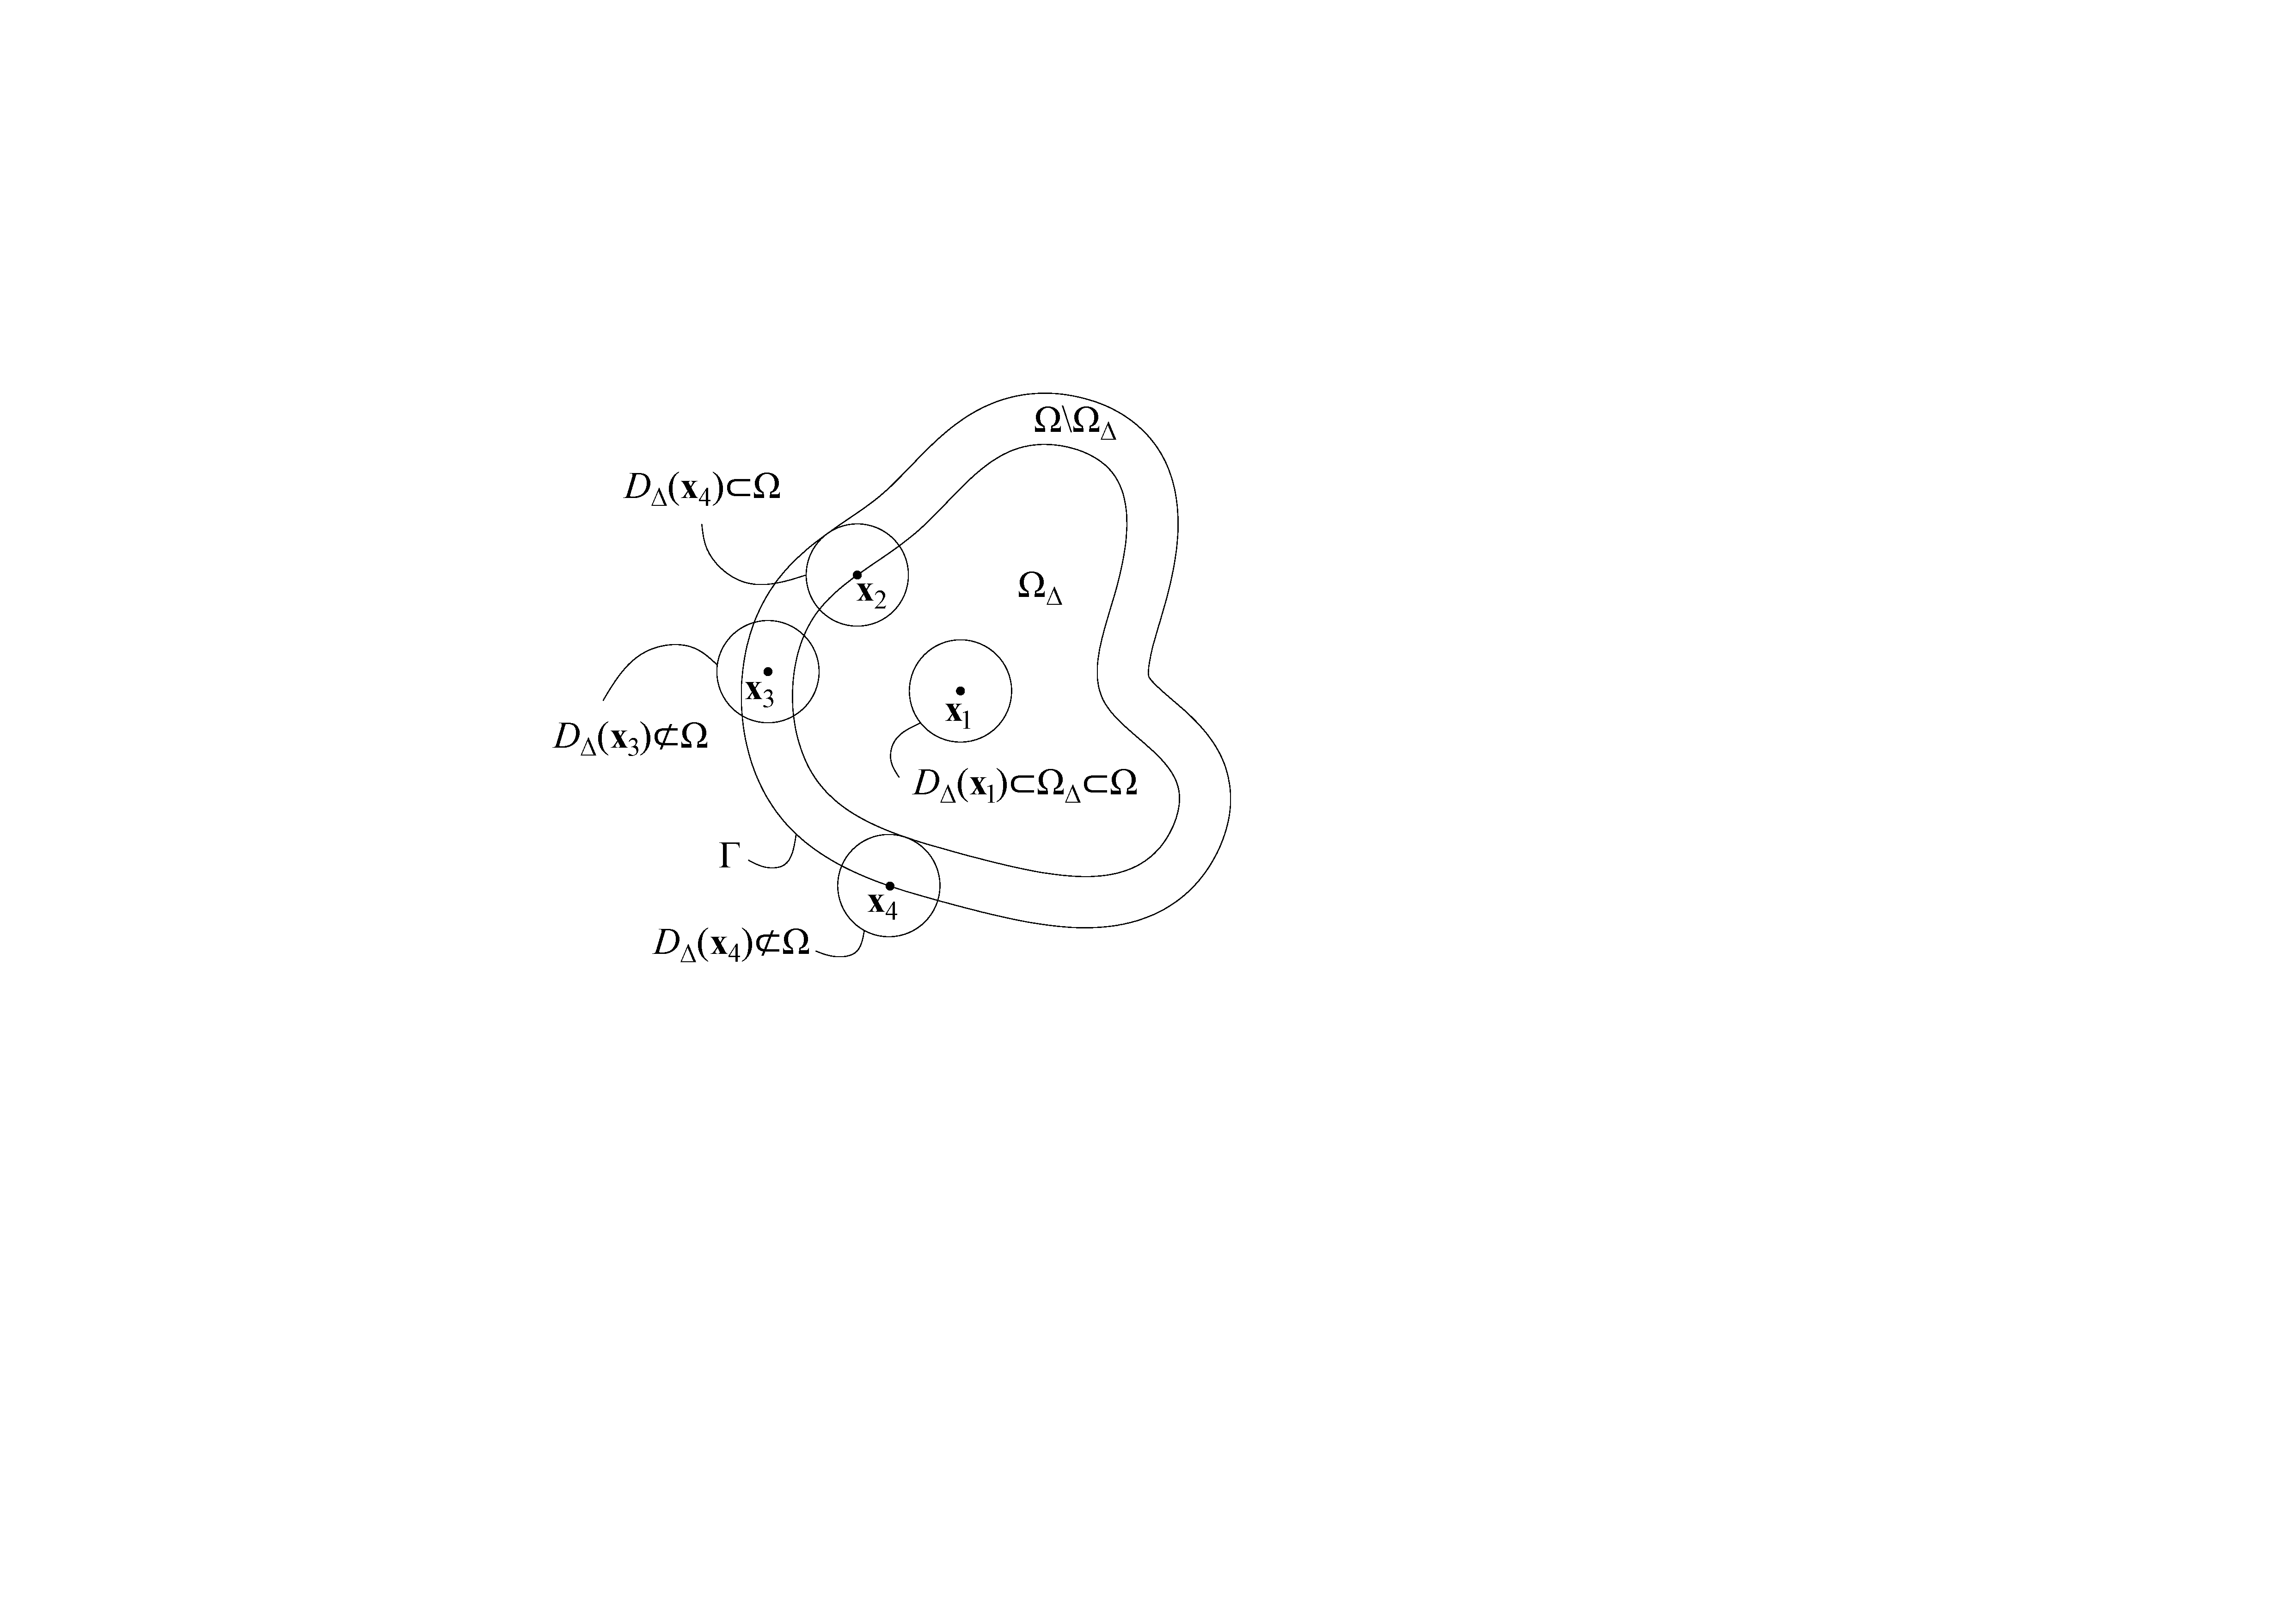
\includegraphics[width=0.5\linewidth]{Figuras/AbrFiltro.pdf}
    \caption{Abrangência do filtro $g$.}
    Fonte: Adaptado de \citeonline{hughes2000large}.
    \label{fig:AbrFiltro}
\end{figure}

%==================================================================================================
\subsection{\textit{Variational Multiscale Methods}} \label{VMS}
%==================================================================================================

O Método Multiescala (VMS) foi introduzido por Hughes e colaboradores \cite{hughes1995multiscale, hughes1996space, hughes1998variational}, onde foi proposta a separação de um problema em dois campos: o campo próximo (\textit{near-field}) e o campo distante (\textit{far-field}). Nesse sentido, o primeiro encontra-se envolto à uma superfície e apresenta escalas pequenas, utilizando-se de uma malha mais refinada para obtenção de resultados, enquanto o segundo apresenta escalas maiores com uma malha mais grosseira.

Esse tipo de análise se mostra promissora ao se estudar problemas em que há a presença de efeitos em diversas escalas, como a formação de camada limite ou de turbulências \cite{fernandes2020tecnica}.

Este método foi utilizado também em problemas envolvendo modelagem em grandes vórtices (VMS-LES) \cite{hughes2000large, bazilevs2007variational}, onde os autores analisaram aproximações a partir das equações de Navier-Stokes incompressíveis, obtendo, assim, resultados favoráveis sobre modelos clássicos de análise LES. Já estudos acerca de escoamentos turbulentos em canais apresentaram bons resultados ao se aplicar essa modelagem \cite{hughes2002variational}.

O VMS consiste na consideração de uma solução tentativa e uma função peso dadas por $\mathcal{V}=\mathcal{V}(\mathrm{Q})$, consideradas idênticas. Com isso, assume-se que existe um $\mathbf{U}=\{\mathbf{u},p\}\in\mathcal{V}$, tal que $\mathbf{u}=\mathbf{0}$ e $\int_{\Omega}{p(t)d\Omega}=0\forall t\in(0,T)$. Assim, deve-se determinar $\mathbf{U}\in\mathcal{V}$ de forma que $\mathbf{W}=\{\mathbf{w},q\}\in\mathcal{V}$. Com isso, aplica-se o método de Galerkin, impondo as condições iniciais de forma a se obter \cite{hughes2002variational}:

\begin{equation}
    B(\mathbf{W},\mathbf{U})=(\mathbf{W},\mathbf{F})\text{,}
    \label{B}
\end{equation}

\noindent em que

\[
B(\mathbf{W},\mathbf{U})=(\mathbf{w}(T^-),\mathbf{u}(T^-))_\Omega
-\left(\frac{\partial\mathbf{w}}{\partial t},\mathbf{u}\right)_\mathrm{Q}
-\left(\mathbf{\nabla}\mathbf{w},\mathbf{u}\otimes\mathbf{u}\right)_\mathrm{Q}\]
\begin{equation}
    +\left(q,\mathbf{\nabla}\cdot\mathbf{u}\right)_\mathrm{Q}
    -\left(\mathbf{\nabla}\cdot w,p\right)_\mathrm{Q}
    +\left(\mathbf{\nabla}^s\mathbf{w},2\nu\mathbf{\nabla}^s\mathbf{u}\right)_\mathrm{Q}\text{, e}
    \label{B-2}
\end{equation}

\begin{equation}
    (\mathbf{W},\mathbf{F})=(\mathbf{w},\mathbf{f})_\mathrm{Q}+(\mathbf{w}(0^+),\mathbf{u}(0^-))_\Omega\text{,}
    \label{WF}
\end{equation}

\noindent sendo o operador $(\cdot,\cdot)_\mathcal{D}$ o produto interno $L_2(\mathcal{D})$, dado por:

\begin{equation}
    (f,g)_\mathcal{D}=\int_\mathcal{D}{fgd\mathcal{D}}\text{,}
    \label{L2}
\end{equation}

\noindent no qual $\mathcal{D}$ pode ser igual a $\Omega$ ou $Q$ e \cite{bazilevs2010large}

\begin{equation}
    \mathbf{\nabla}^s(\mathbf{\cdot})=\frac{1}{2}(\mathbf{\nabla}(\mathbf{\cdot})+\mathbf{\nabla}(\mathbf{\cdot})^T)
    \label{nablas}
\end{equation}

\noindent é o gradiente simétrico de um vetor, que pode ser $\mathbf{u}$ ou $\mathbf{w}$.

A separação das escalas é feita como:

\begin{equation}
    \mathcal{V}=\bar{\mathcal{V}}\oplus\mathcal{V}'\text{,}
    \label{SepV}
\end{equation}

\noindent em que $\bar{\mathcal{V}}$ representa um espaço de grandes escalas e de dimensões finitas, enquanto $\mathcal{V}'$ representa um espaço de pequenas escalas de infinitas dimensões, as quais podem ser substituídas por um espaço de dimensões finitas em um modelo discreto. Nesse sentido, pode-se considerar que $\mathcal{V}'$ é um enriquecimento de $\bar{\mathcal{V}}$.

Assim, a partir das equações \ref{SepV} e \ref{B-2} obtém-se que:

\begin{equation}
    B(\bar{\mathbf{W}},\bar{\mathbf{U}}+\mathbf{U}')=(\bar{\mathbf{W}},\mathbf{F})\text{, e}
    \label{B-3}
\end{equation}

\begin{equation}
    B(\mathbf{W}',\bar{\mathbf{U}}+\mathbf{U}')=(\mathbf{W}',\mathbf{F})\text{,}
    \label{B-4}
\end{equation}

\noindent em que

\begin{equation}
    \mathbf{U}=\bar{\mathbf{U}}+\mathbf{U}'\text{, e}
    \label{U}
\end{equation}

\begin{equation}
    \mathbf{W}=\bar{\mathbf{W}}+\mathbf{W}'\text{,}
    \label{W}
\end{equation}

\noindent tais que $\bar{\mathbf{U}},\bar{\mathbf{W}}\in\bar{\mathcal{V}}$ e $\mathbf{U}',\mathbf{W}'\in\mathcal{V}'$.

Dessa forma, toma-se $B_1$ como o operador linearizado de Navier-Stokes, dado por:

\[B_1(\mathbf{W},\bar{\mathbf{U}},\mathbf{U}')=\left.\frac{d}{d\varepsilon}B(\mathbf{W},\bar{\mathbf{U}}+\varepsilon\mathbf{U}')\right|_{\varepsilon=0}
=(\mathbf{w}(T^-),\mathbf{u}'(T^-))_\Omega
-\left(\frac{\partial\mathbf{w}}{\partial t},\mathbf{u}'\right)_\mathrm{Q}\]
\begin{equation}
    -(\mathbf{\nabla}\mathbf{w},\bar{\mathbf{u}}\otimes\mathbf{u}'+\mathbf{u}'\otimes\bar{\mathbf{u}})_\mathrm{Q}
    +(q,\mathbf{\nabla}\cdot\mathbf{u}')_\mathrm{Q}
    -(\mathbf{\nabla}\cdot\mathbf{w},p')_\mathrm{Q}
    +(\mathbf{\nabla}^s\mathbf{w},2\nu\mathbf{\nabla}^s\mathbf{u}')_\mathrm{Q}
    \text{.}
    \label{B_1}
\end{equation}

Com isso, pode-se escrever $B(\mathbf{W},\bar{\mathbf{U}}+\mathbf{U}')$ como:

\begin{equation}
    B(\mathbf{W},\bar{\mathbf{U}}+\mathbf{U}')=B(\mathbf{W},\bar{\mathbf{U}})+B_1(\mathbf{W},\bar{\mathbf{U}},\mathbf{U}')+\frac{1}{2}B_2(\mathbf{W},\bar{\mathbf{U}},\mathbf{U}')\text{,}
    \label{B-5}
\end{equation}

\noindent sendo:

\begin{equation}
    \frac{1}{2}B_2(\mathbf{W},\bar{\mathbf{U}},\mathbf{U}')=\frac{1}{2}\left.\frac{d^2}{d\varepsilon^2}B(\mathbf{W},\bar{\mathbf{U}}+\varepsilon\mathbf{U}')\right|_{\varepsilon=0}=-(\mathbf{\nabla}\mathbf{w},\mathbf{u}'\otimes\mathbf{u}')_\mathrm{Q}\text{.}
    \label{B_2}
\end{equation}

Assim, é possível reescrever as equações \ref{B-3} e \ref{B-4} como:

\begin{equation}
    B(\bar{\mathbf{W}},\bar{\mathbf{U}})+B_1(\bar{\mathbf{W}},\bar{\mathbf{U}},\mathbf{U}')=(\mathbf{\nabla}\bar{\mathbf{w}},\mathbf{u}'\otimes\mathbf{u}')_\mathrm{Q}+(\bar{\mathbf{W}},\mathbf{F})\text{, e}
    \label{B-6}
\end{equation}

\begin{equation}
    B_1(\bar{\mathbf{W}},\bar{\mathbf{U}},\mathbf{U}')-(\mathbf{\nabla}\mathbf{w},\mathbf{u}'\otimes\mathbf{u}')_\mathrm{Q}=-[B(\mathbf{W}',\bar{\mathbf{U}})-(\mathbf{W}',\mathbf{F})]\text{,}
    \label{B-7}
\end{equation}

\noindent que equivalem a duas equações não-lineares que, ao se conhecer os valores referentes às pequenas escalas, é possível determinar os valores referentes às grandes escalas \cite{hughes2002variational}.

%==================================================================================================
\subsection{\textit{Remeshing} e enriquecimento} \label{ReE}
%==================================================================================================

%==================================================================================================
\subsection{\textit{Reynolds-Averaged Navier-Stokes}} \label{RANS}
%==================================================================================================

Na tentativa de se obter soluções aproximativas para as equações de Navier-Stokes, são desenvolvidas técnicas de aproximação, baseadas em equações diferenciais. Uma dessas aproximações, denominada de \textit{Reynolds-Averaged Navier-Stokes} (RANS) busca encontrar uma solução a partir da decomposição de Reynolds. Nesse contexto, observa-se que simulações feitas utilizando RANS são mais eficientes computacionalmente que aquelas feitas a partir de LES, além de possuirem uma implmentação mais facilitada \cite{alfonsi2009reynolds, ling2015evaluation}. Ainda segundo \citeonline{alfonsi2009reynolds}, problemas envolvendo RANS podem ser classificados dependendo da quantidade de equações diferenciais resolvidas, em que cada equação adicionada refere-se ao transporte de uma propriedade relativa à turbulência.

Sua obtenção parte da equação \ref{Sist1} e considera-se que a velocidade $\mathbf{u}$ pode ser decomposto em duas parcelas: uma devida à velocidade média $\bar{\mathbf{u}}$ e uma devida à flutuações de velocidade $\mathbf{u}'$, ou seja, $\mathbf{u}=\bar{\mathbf{u}}+\mathbf{u}'$. Sendo assim, a velocidade média é obtida como:

\begin{equation}
    \bar{\mathbf{u}}=\lim_{T\to\infty}{\frac{1}{T}\int_{t_0}^{t_0+T}{\mathbf{u}dt}}\text{.}
    \label{umed}
\end{equation}

\noindent Também vale ressaltar que, dessa forma, a média das flutuações de velocidades deve ser nula.

Assim, reescrevendo a equação \ref{Sist1} em termos de parcelas médias e flutuações e utilizando a notação indicial, tem-se que:

\begin{equation}
    \frac{\partial(\bar{u}_i+u_i')}{\partial t}+\frac{\partial((\bar{u}_i+u_i')(\bar{u}_j+u_j'))}{\partial y_j}+\frac{1}{\rho}\frac{\partial(\bar{p}+p')}{\partial y_i}=\nu\frac{\partial^2(\bar{u}_j+u_j')}{\partial y_j\partial y_i}+\frac{\bar{b}_i+b'_i}{\rho}\text{.}
    \label{RANS1}
\end{equation}

Aplicando uma variação média em cada termo da equação \ref{RANS1} obtém-se:

\begin{equation}
    \overline{\frac{\partial(\bar{u}_i+u_i')}{\partial t}}+\overline{\frac{\partial((\bar{u}_i+u_i')(\bar{u}_j+u_j'))}{\partial y_j}}+\overline{\frac{1}{\rho}\frac{\partial(\bar{p}+p')}{\partial y_i}}=\overline{\nu\frac{\partial^2(\bar{u}_j+u_j')}{\partial y_j\partial y_i}}+\overline{\frac{\bar{b}_i+b'_i}{\rho}}\text{.}
    \label{RANS2}
\end{equation}

Já que a aplicação de variações média envolve integração temporal, a derivada em realação a $t$ pode ser eliminada. Assim, sabendo-se que:

\begin{equation}
    \frac{\bar{u}_i}{\partial x_i}=0\text{,}
    \label{dudxi}
\end{equation}

\noindent é possível realizar algumas simplificações na equação \ref{RANS2}, o que resulta em:

\begin{equation}
    \bar{u}_j\frac{\partial\bar{u}_i}{\partial y_j}+\frac{\partial\overline{u_i'u_j'}}{\partial y_j}+\frac{1}{\rho}\frac{\partial\bar{p}}{\partial y_i}=\nu\frac{\partial^2\bar{u}_j}{\partial y_j\partial y_i}+\frac{\bar{b}_i}{\rho}\text{, ou}
    \label{RANS3}
\end{equation}

\begin{equation}
    \bar{u}_j\frac{\partial\bar{u}_i}{\partial y_j}=\frac{\bar{b}_i}{\rho}+\frac{\partial}{\partial y_j}\left[\nu\frac{\partial\bar{u}_j}{\partial y_i}-\frac{\bar{p}}{\rho}\delta_{ij}-\overline{u_i'u_j'}\right]\text{.}
    \label{RANS4}
\end{equation}

Já, de forma mais genérica, a equação \ref{RANS4} pode ser escrita de forma a descrever a evolução temporal:

\[
    \frac{\partial\overline{u_i'u_j'}}{\partial t}
    +\bar{u}_k\frac{\partial{\overline{u_i'u_j'}}}{\partial y_k}
    =-\overline{u_i'u_k'}\frac{\partial\bar{u}_i}{\partial y_k}
    -\overline{u_j'u_k'}\frac{\partial\bar{u}_i}{\partial y_k}
    +\overline{\frac{p'}{\rho}\left(\frac{\partial u_i'}{\partial y_j}+\frac{\partial u_j'}{\partial y_i}\right)}
    \]
\begin{equation}
    -\frac{\partial}{\partial y_k}\left(\overline{u_i'u_j'u_k'}+\frac{\overline{p'u_i'}}{\rho}\delta_{jk}+\frac{\overline{p'u_j'}}{\rho}\delta_{ik}-\nu\frac{\partial\overline{u_i'u_j'}}{\partial y_k}\right)
    -2\nu\overline{\frac{\partial u_i'}{\partial y_k}\frac{\partial u_j'}{\partial y_k}}
    \text{.}
    \label{RANS5}
\end{equation}

\end{document}